\documentclass[10pt,a4paper]{article}
\usepackage[latin1]{inputenc}
\usepackage{amsmath}
\usepackage{amsfonts}
\usepackage{amssymb}
\usepackage{graphics} 
\usepackage{graphicx}
\usepackage{float}
\usepackage{subfigure}

\author{Ana Huaman}
\title{\textbf{CS 7785 Assignment} \\ Module: Nonlinear Control}

\begin{document}
\maketitle

\textbf{Note:} The pdf version of this document has been submitted on T-Square (if you are reading the paper version) with the plots in color. Thanks!

\section*{Problem 1}
Recall the 3R manipulator (three revolute joint) depicted in Figure 1, that I gave as an example of feedback linearization. Well, it is time to follow through on my lectures and check it out for yourself. This problem will focus on seeing how the different types of controllers work. The code stub is available for download from the course website, and needs to be modified to get the simulations that are required below. All you have to do is fill out the control variables in the function eom1a, eom1b and eom1c. We want to compare the three similar control strategies.

\begin{figure}[hb]
  \centering
  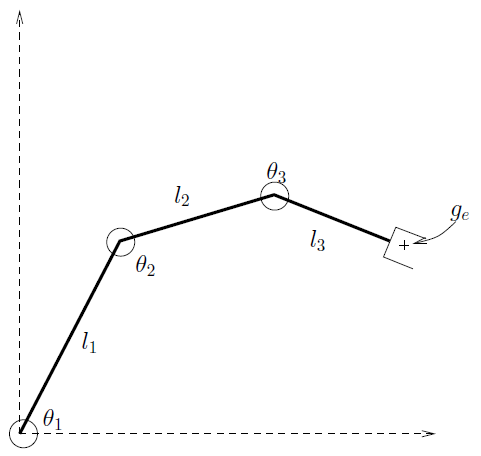
\includegraphics[angle = 0, scale = 0.3]{figures/manipulator3R.png} 
  \label{fig:manipulator3R}
  \caption{3R Manipulator}
\end{figure}

\subsection*{(a)}
Run the simulation to convergence with the initial condition $\theta = (0,0,0)^{T}$ and $\dot{\theta} = (0,0,0)^{T}$. Let there be a control torque that tries to stabilize the system to $\theta^{*} = ( \dfrac{\pi}{8}, \dfrac{\pi}{5}, -\dfrac{\pi}{8})^{T}$ and zero joint velocity. Use the most simplest control law discussed in class.

\[ \tau = -K_{p}e - K_{v}\dot{\theta} \]

Choose $K_{p} = I$ and $K_{v} = 3I$ where $I$ is the identity matrix. Plot the evolution of $\theta$ in one graph and $\dot{\theta}$ in another. How long did it take to converge to within about $10\%$ error?

\subsubsection*{Answer}
Modifying the script we get the plots shown below. The time required to converge to about $10\%$ error was 40.41 seconds, as it can be seen more clearly in Fig. \ref{fig:Q1aErrors}

\begin{figure}[H]
  \centering
  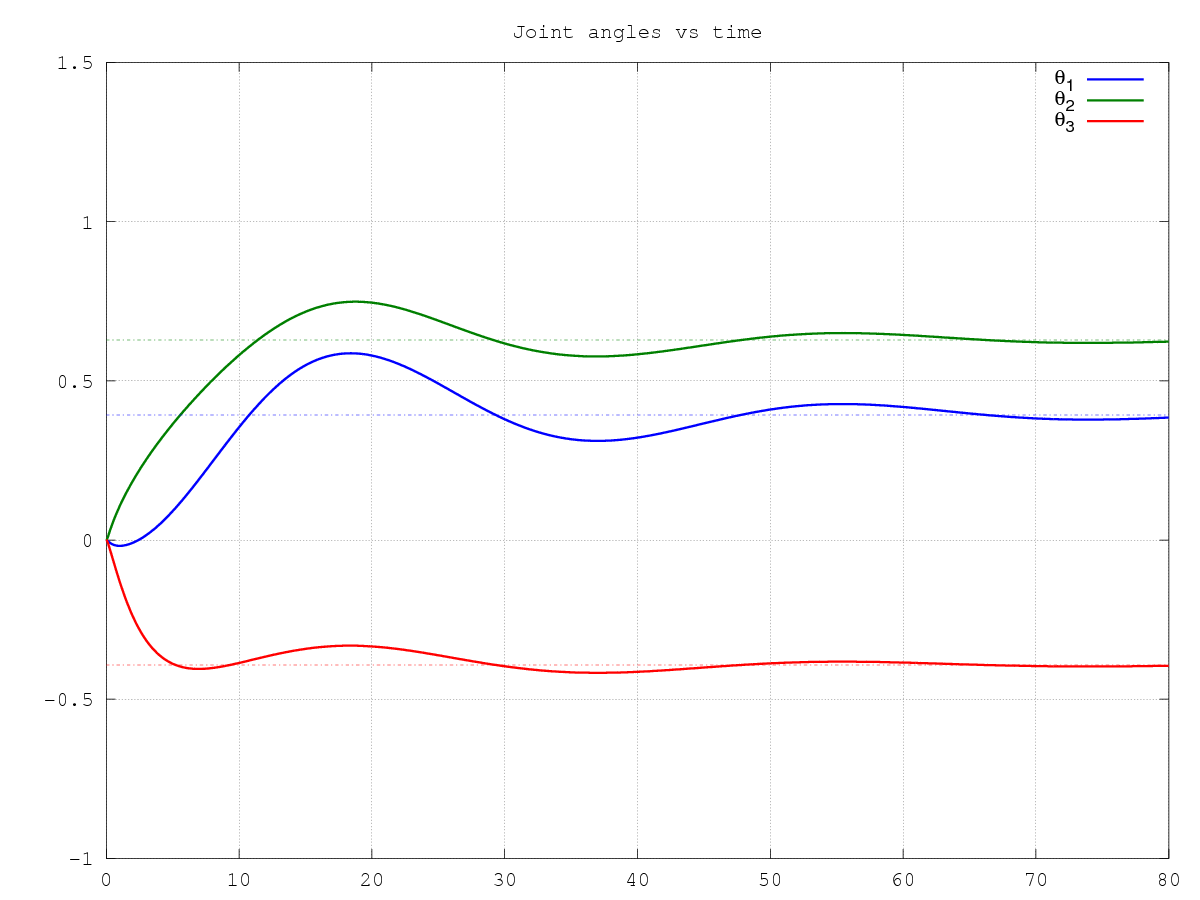
\includegraphics[angle = 0, scale = 0.3]{figures/Question1aJoints.png} 
  \label{fig:Q1aJoints}
  \caption{$\theta$ vs $t$}
\end{figure}

\begin{figure}[H]
  \centering
  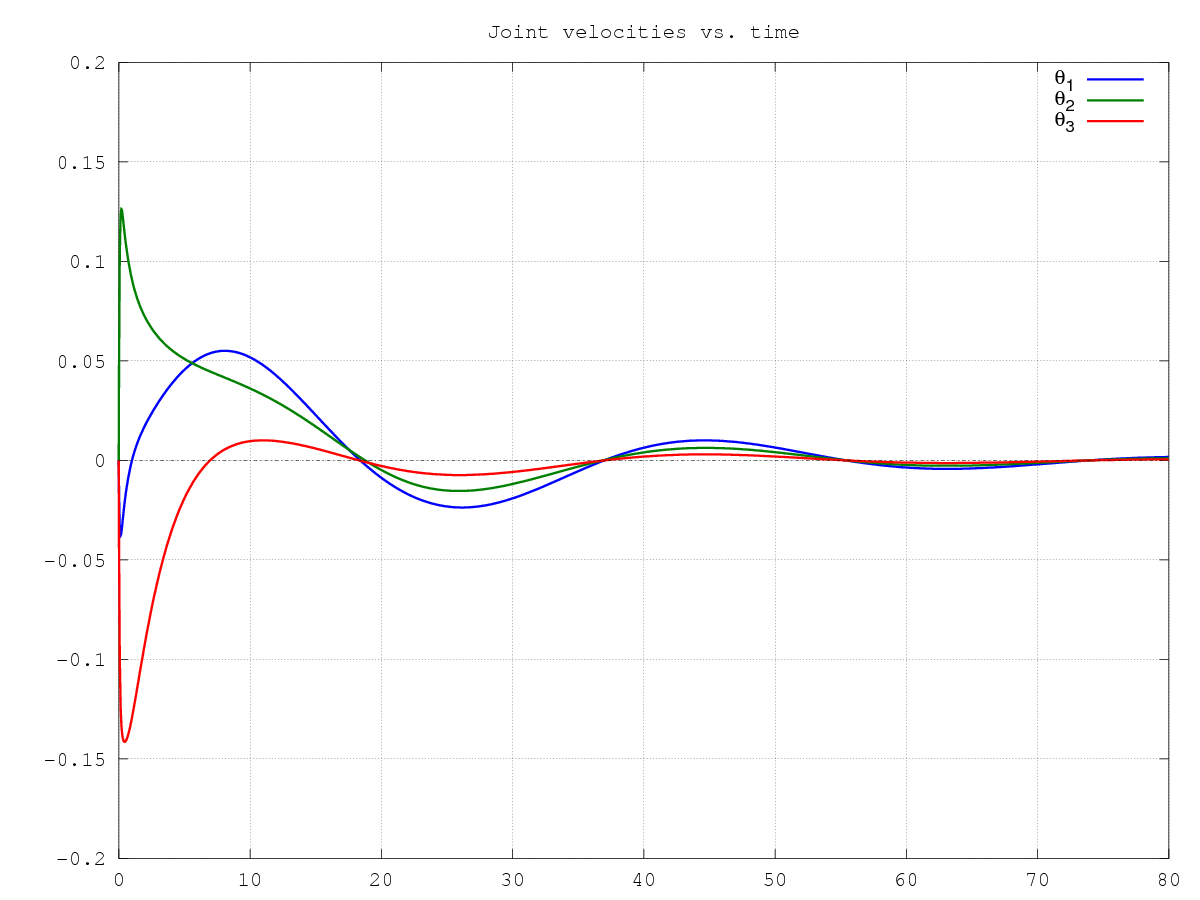
\includegraphics[angle = 0, scale = 0.3]{figures/Question1aVels.png} 
  \label{fig:Q1aVels}
  \caption{$\dot{\theta}$ vs $t$}
\end{figure}

\begin{figure}[H]
  \centering
  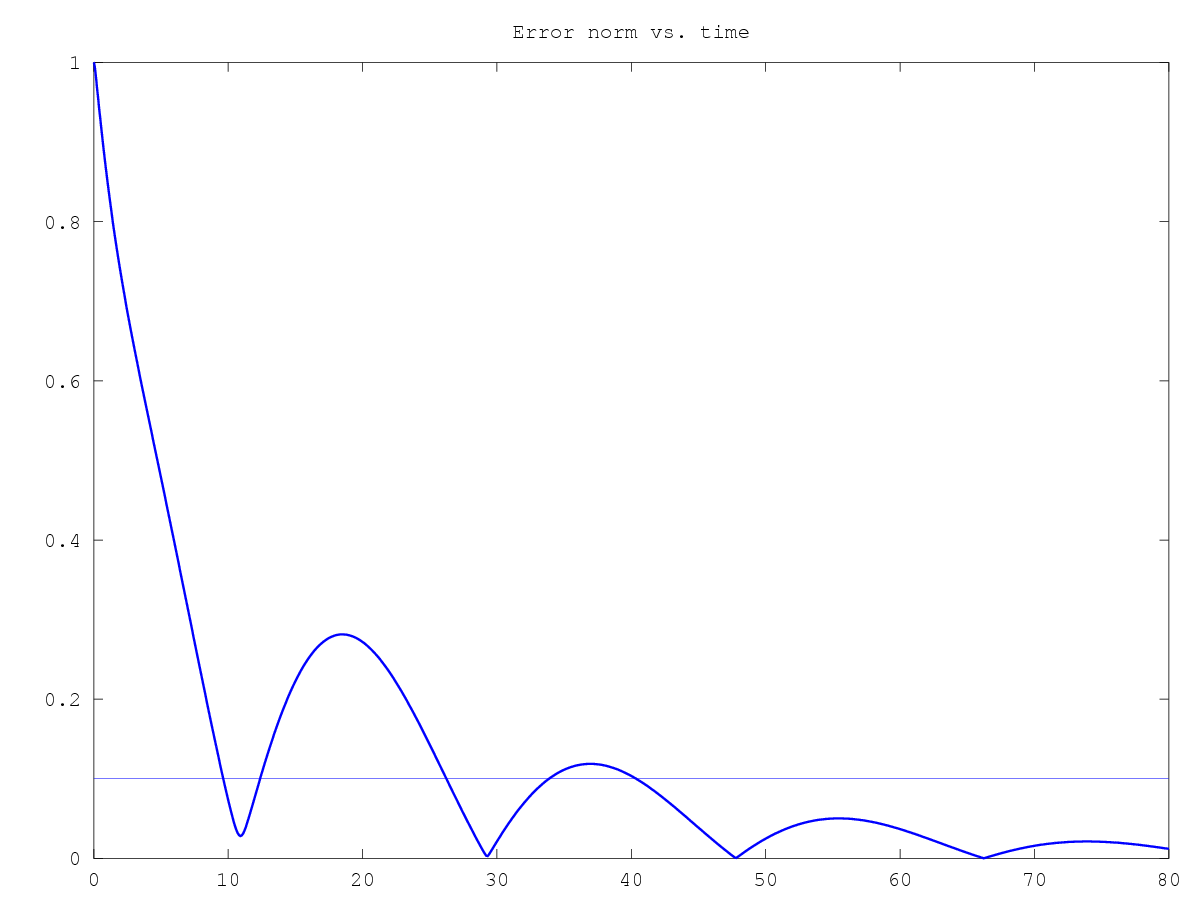
\includegraphics[angle = 0, scale = 0.3]{figures/Question1aErrors.png} 
  \label{fig:Q1aErrors}
  \caption{$e$ vs $t$}
\end{figure}


\subsection*{(b)}
Do the same as in part (a) but with the more sophisticated controller that tries to invert out some of the dynamics

\[ \tau = \tilde{M}(\theta)\left ( -K_{p}e - K_{v}\dot{\theta} \right ) \]

where $\tilde{M}$ is just the diagonal part of the true mass matrix. Choose $K_{p} = I$ and $K_{v} = 3I$ where $I$ is the identity matrix. Plot the evolution of $\theta$ in one graph and $\dot{\theta}$ in another. How long did it take to converge to within about $10\%$ error?
\subsubsection*{Answer}
Modifying the script we get the plots shown below. The time required to converge to about $10\%$ error was 7.13 seconds, as it can be seen more clearly in Fig. \ref{fig:Q1bErrors}

\begin{figure}[H]
  \centering
  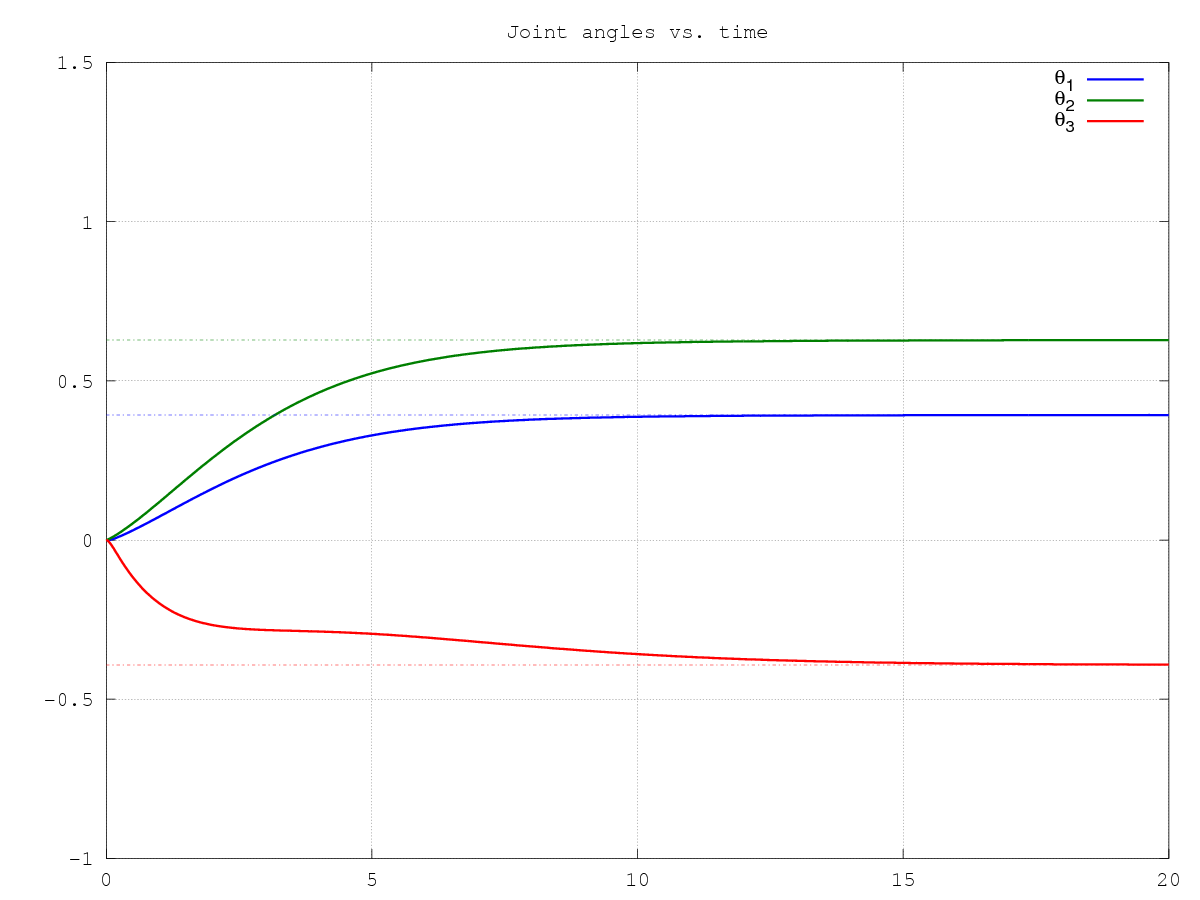
\includegraphics[angle = 0, scale = 0.3]{figures/Question1bJoints.png} 
  \label{fig:Q1bJoints}
  \caption{$\theta$ vs $t$}
\end{figure}

\begin{figure}[H]
  \centering
  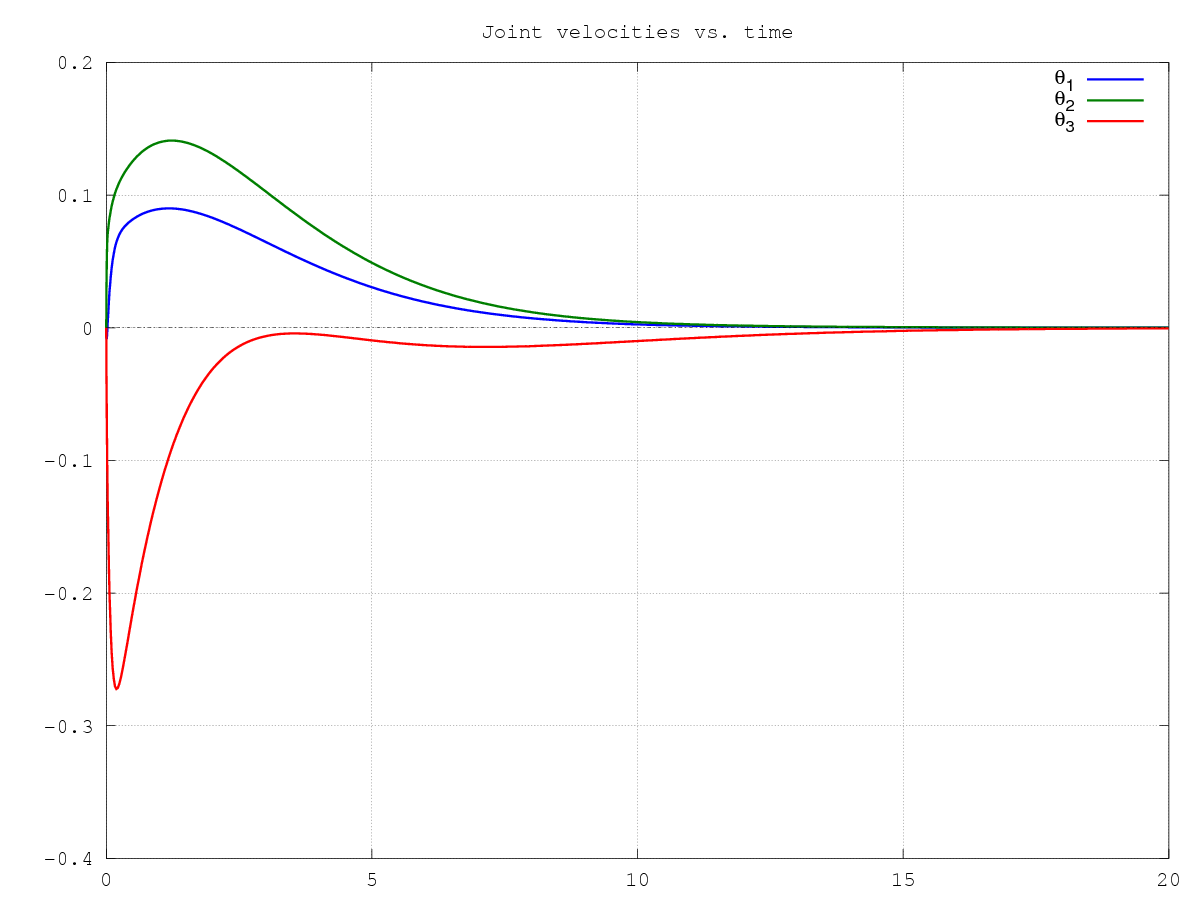
\includegraphics[angle = 0, scale = 0.3]{figures/Question1bVels.png} 
  \label{fig:Q1bVels}
  \caption{$\dot{\theta}$ vs $t$}
\end{figure}

\begin{figure}[H]
  \centering
  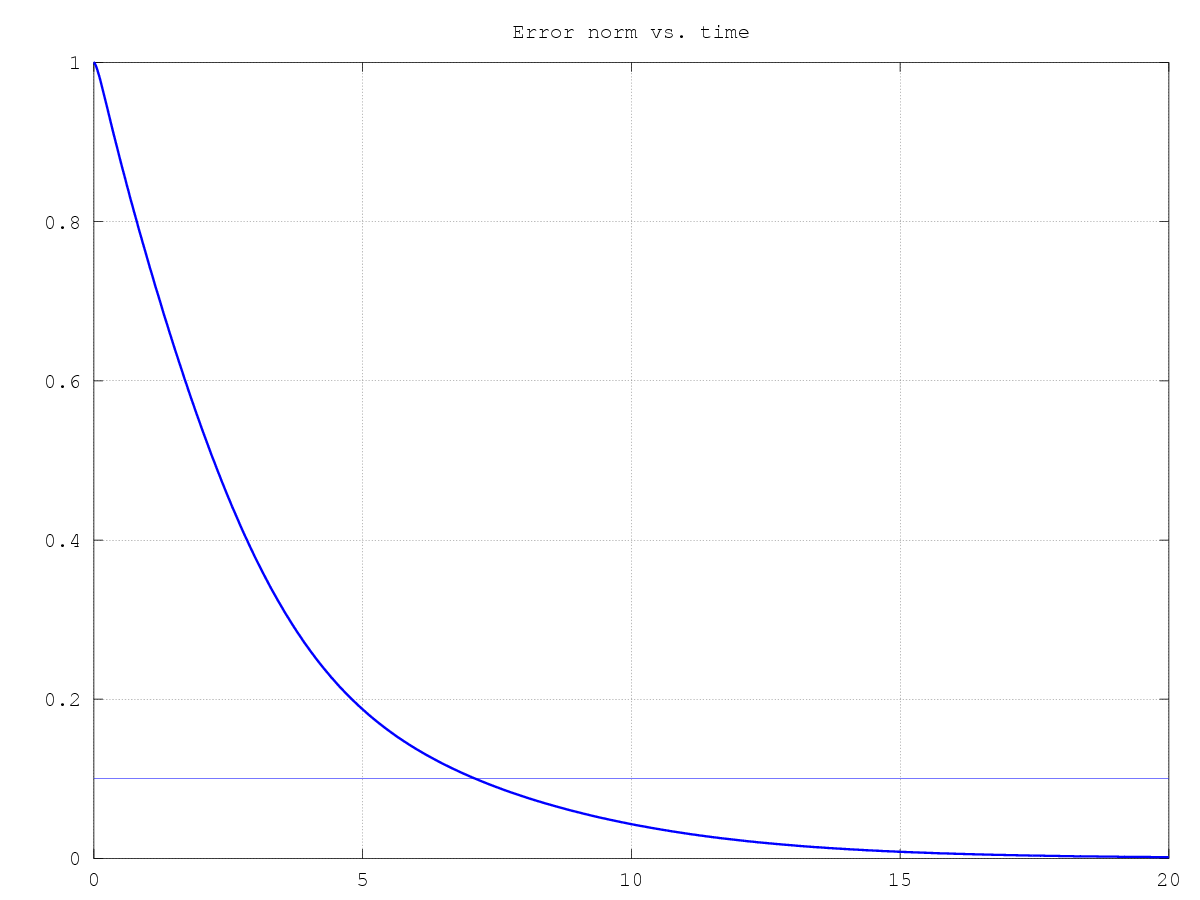
\includegraphics[angle = 0, scale = 0.3]{figures/Question1bErrors.png} 
  \label{fig:Q1bErrors}
  \caption{$e$ vs $t$}
\end{figure}


\subsection*{(c)}
Do the same as in part (a) but with the more sophisticated controller that tries to invert out some of the dynamics

\[ \tau = M(\theta)\left ( -K_{p}e - K_{v}\dot{\theta} \right )  + C(\theta, \dot{\theta})\dot{\theta} + N(\theta, \dot{\theta}) \]

Choose $K_{p} = I$ and $K_{v} = 3I$ where $I$ is the identity matrix. Plot the evolution of $\theta$ in one graph and $\dot{\theta}$ in another. How long did it take to converge to within about $10\%$ error?

\subsubsection*{Answer}
Modifying the script we get the plots shown below. The time required to converge to about $10\%$ error was 6.49 seconds, as it can be seen more clearly in Fig. \ref{fig:Q1aErrors}

\begin{figure}[H]
  \centering
  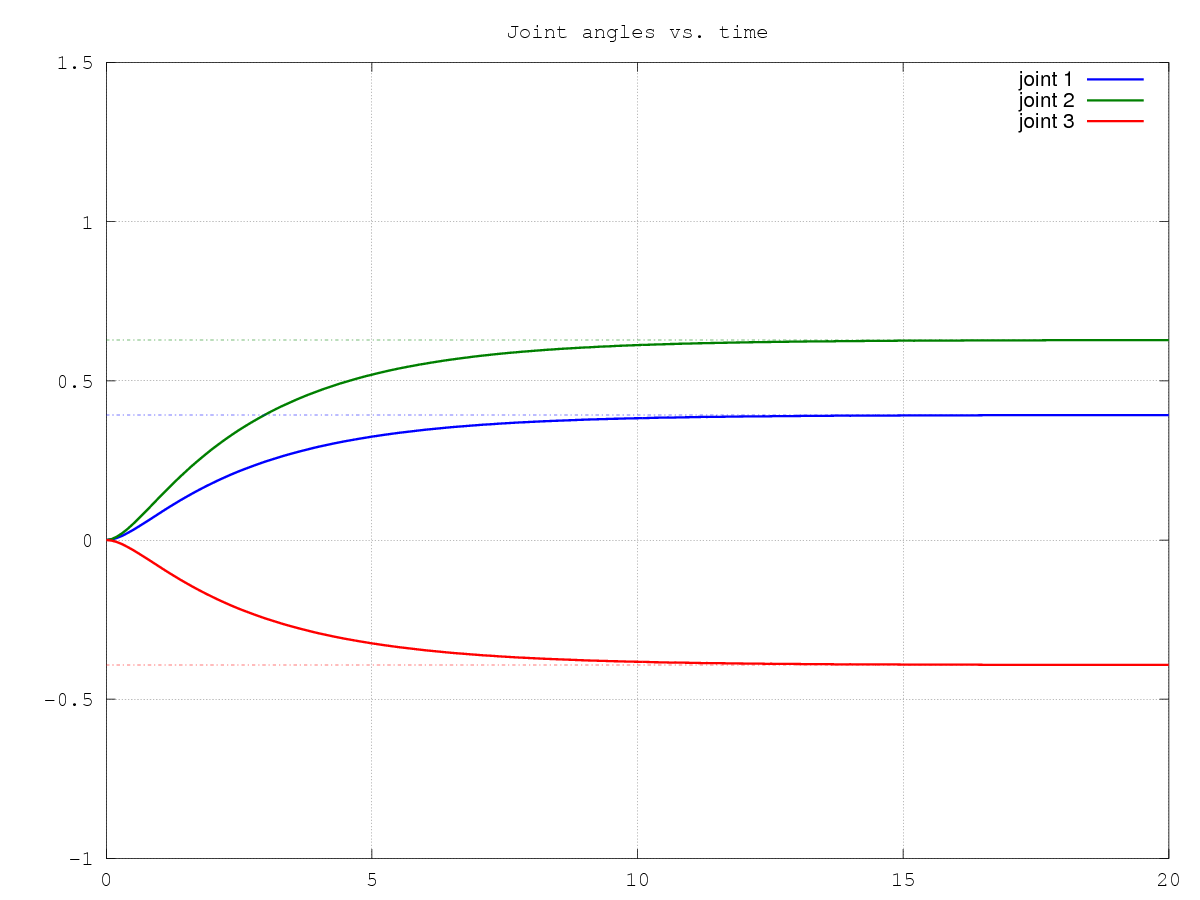
\includegraphics[angle = 0, scale = 0.3]{figures/Question1cJoints.png} 
  \label{fig:Q1cJoints}
  \caption{$\theta$ vs $t$}
\end{figure}

\begin{figure}[H]
  \centering
  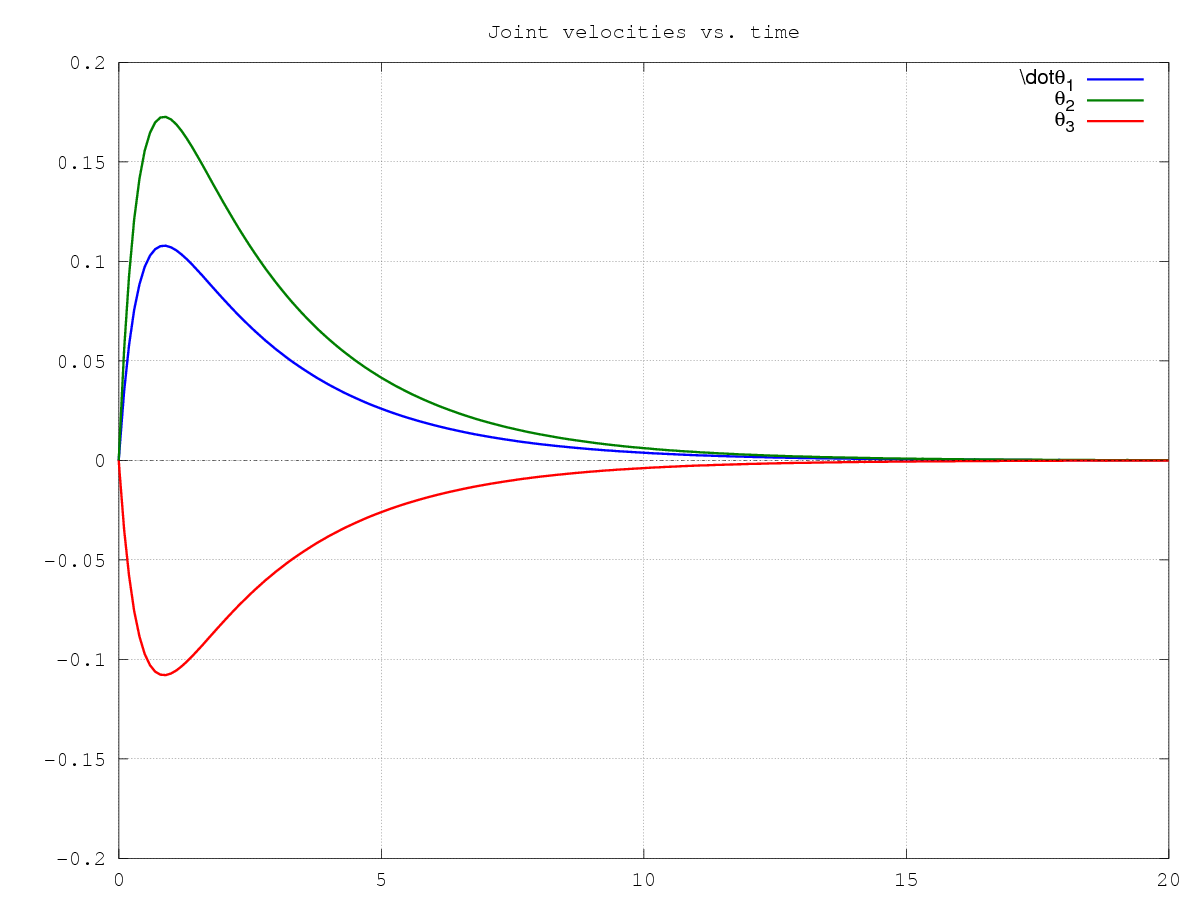
\includegraphics[angle = 0, scale = 0.3]{figures/Question1cVels.png} 
  \label{fig:Q1cVels}
  \caption{$\dot{\theta}$ vs $t$}
\end{figure}

\begin{figure}[H]
  \centering
  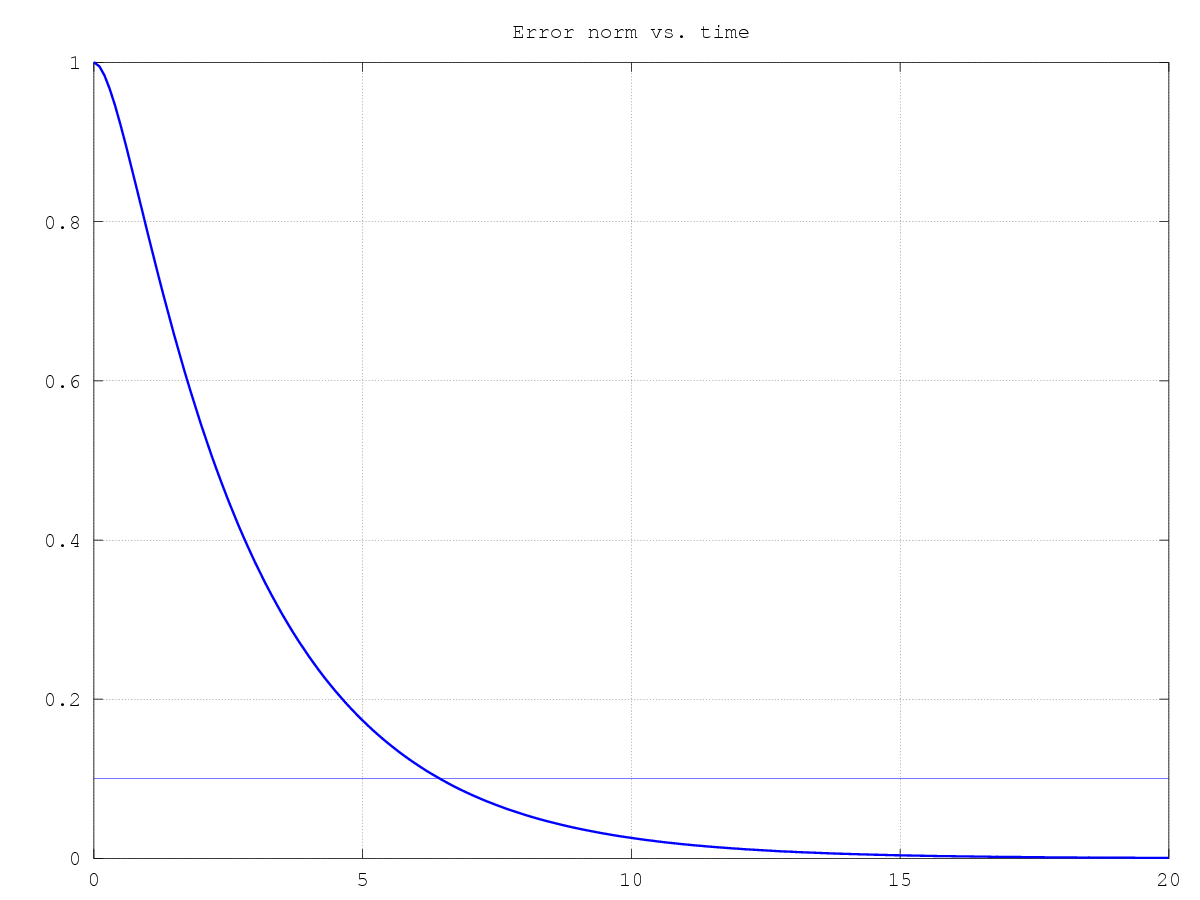
\includegraphics[angle = 0, scale = 0.3]{figures/Question1cErrors.png} 
  \label{fig:Q1cErrors}
  \caption{$e$ vs $t$}
\end{figure}

% --------------------------------
\section*{Problem 2}
This homework problem asks for you to actually implement the position-stabilizing controller for the car-like vehicle. It is not as bad as it looks from all of the math. The equation of motion in coordinate form are:

\[ \begin{Bmatrix}
   \dot{x} \\
   \dot{y} \\
   \dot{\theta} 
   \end{Bmatrix}
   =
  \begin{bmatrix}
  \cos (\theta) & 0 \\
  \sin (\theta) & 0 \\
  0 & 1
  \end{bmatrix}  
  \begin{Bmatrix}
  \nu \\
  \omega
  \end{Bmatrix}
\]

The position-stabilizing controller that we derived required first extending the state to include the transformation parameter $\lambda$

\[ \begin{Bmatrix}
   \dot{x} \\
   \dot{y} \\
   \dot{\theta} \\
   \dot{\lambda}
   \end{Bmatrix}
   =
   \begin{Bmatrix}
   0 \\
   0 \\
   0 \\
   -c(\lambda - \epsilon)\\
   \end{Bmatrix}   
   +
  \begin{bmatrix}
  \cos (\theta) & 0 \\
  \sin (\theta) & 0 \\
  0 & 1 \\
  0 & 0 
  \end{bmatrix}  
  \begin{Bmatrix}
  \nu \\
  \omega
  \end{Bmatrix}
\]

and the actual control law was defined to be

\[ u = R^{-1}_{\lambda} \upsilon + e_{1}\dot{\lambda} \]

where
\begin{center}
$ R_{\lambda} = 
  \begin{bmatrix}
  \cos (\theta) & -\lambda \sin (\theta) \\
  \sin (\theta) & \lambda \cos (\theta) \\
  0 & 1 \\
  0 & 0 
  \end{bmatrix}$ 
and
$e_{1} = 
\begin{Bmatrix}
1 \\
0
\end{Bmatrix}$
\end{center}

with 
\[ \upsilon = -Kz \]

for some $K$ such that $K + K^{T} > 0$ (positive definite) and where $z$ is defined to be
\begin{center}
$z = 
\begin{Bmatrix}
x \\
y
\end{Bmatrix}
+
\lambda Re_{1}$, for 
$ R = 
\begin{bmatrix}
  \cos (\theta) & -\sin (\theta) \\
  \sin (\theta) & \cos (\theta) \\
\end{bmatrix}$
\end{center} 

It may seem complicated but it is just a succesion of simple substitutions.The best thing is to have the code follow exactly the math and it should work out OK.

If you have any questions, feel free to email or drop by.

\subsection*{(a)}
Perform the numerical integration with the initial condition $x_{0} = [-1;2.5;\dfrac{\pi}{2}; 0.2]$ and hand in the parametric plot of the trajectory (x vs y plots)
\subsubsection*{Answer}
The file used to generate this plot is attached to this submission. The plot is shown below. To calculate the states, we used the following control values:

\[ K = \begin{bmatrix}
   1 & 0 \\
   0 & 1 
   \end{bmatrix} \]
\[ c = 1 \]
\[ e = 0.01 \]

\begin{figure}[H]
  \centering
  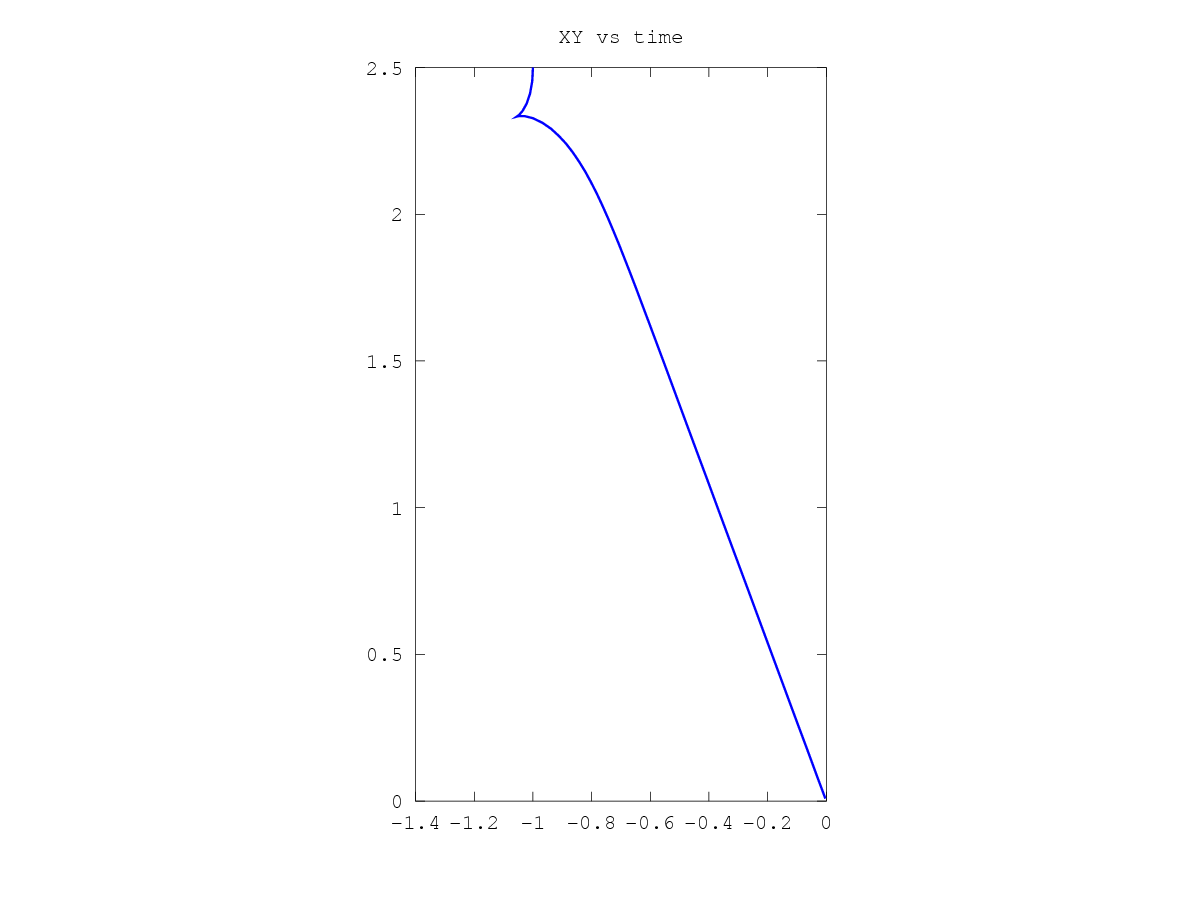
\includegraphics[angle = 0, scale = 0.4]{figures/Question2aXyt.png} 
  \label{fig:Q2aTrajectory}
  \caption{$e$ vs $t$}
\end{figure}


\subsection*{(b)}
Play around with the initial conditions and see how it works. Turn in two additional plots that you found interesting and tell me the initial conditions.
\subsubsection*{Answer}

\textbf{Initial Conditions 1:} $x_{0} = 2.0$, $y_{0} = 3.0$, $\theta = \pi / 4 $, $\lambda_{0} = 3.0$
Here we try with an exaggerated high value of $\lambda$. The result is a trajectory with a very ugly spike. Here the plots
	\begin{figure}[h]
			\centering
			  \subfigure[Parametric trajectory]{
			  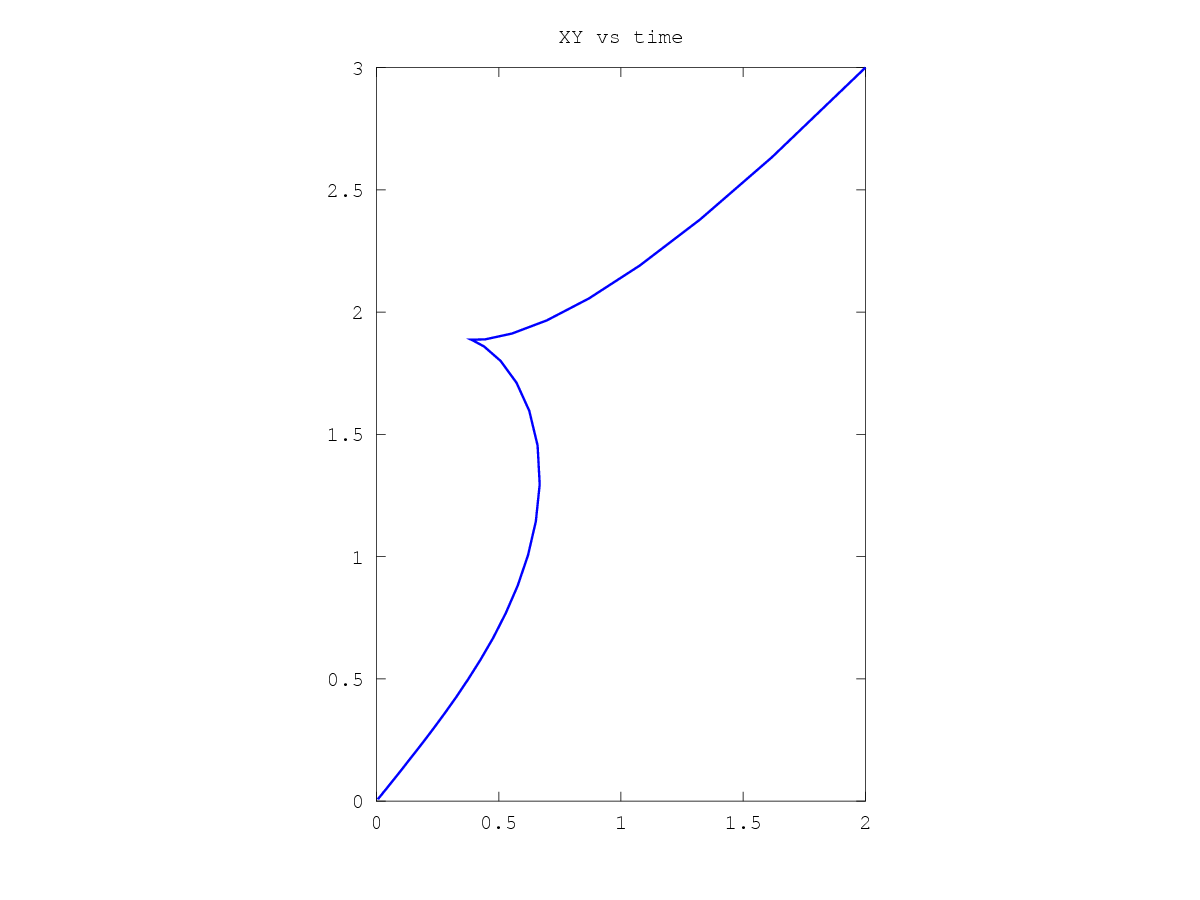
\includegraphics[scale=0.4]{figures/Question2b1Xyt.png} 
	          \label{fig:Q2b1Traj}
              }
              \subfigure[$x$ vs $t$ and $y$ vs $t$ ]{
	          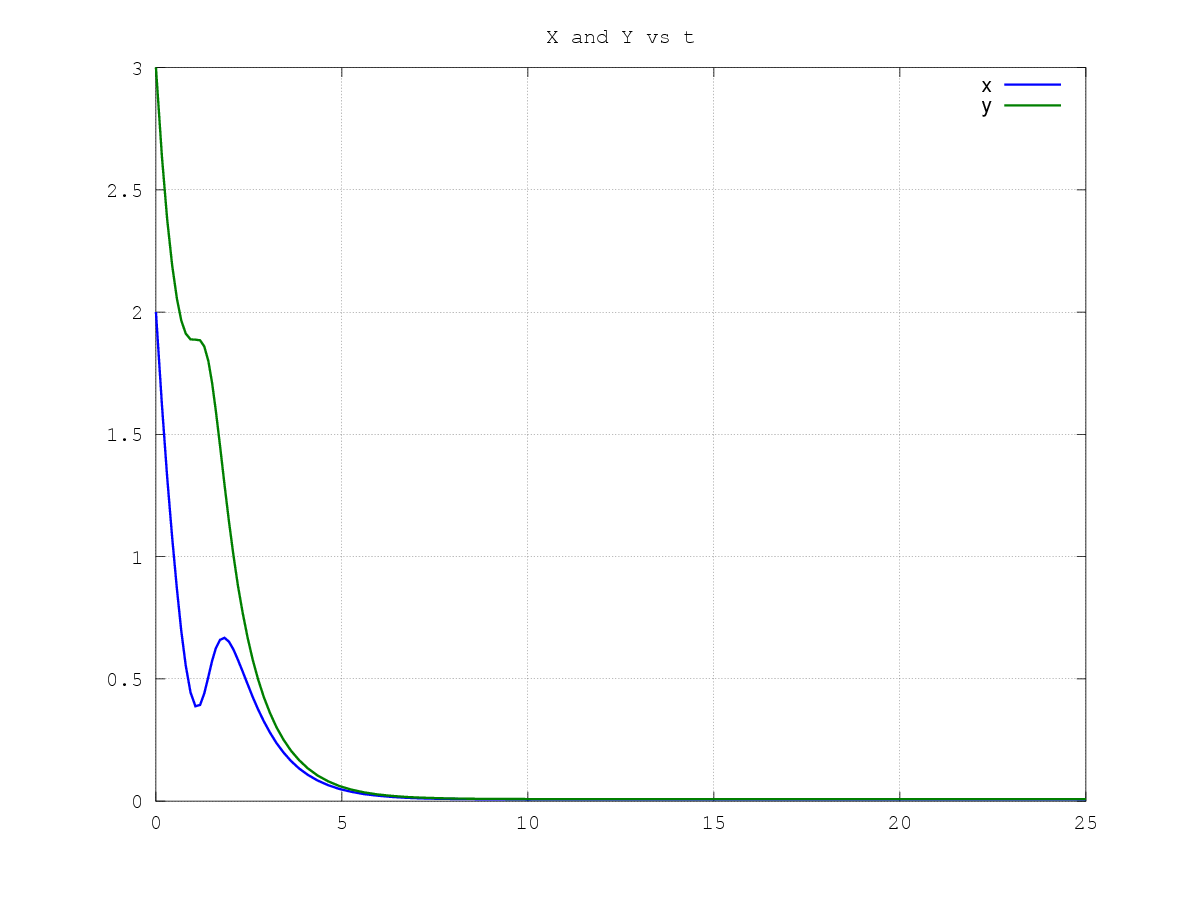
\includegraphics[scale=0.4]{figures/Question2b1Param.png} 	
	          \label{fig:Q2b1Xy}
              } 
            \caption{ Interesting Trajectory 1 }
            \label{fig:Q2b1}
	\end{figure}

% ---------------
\textbf{Initial Conditions 2:} $x_{0} = 2.0$, $y_{0} = 3.0$, $\theta = \pi / 4 $, $\lambda_{0} = 0.05$
Here we try with a smaller $\lambda$. The result is a smoother path (compared with the one above). The plots below. 

	\begin{figure}[h]
			\centering
			  \subfigure[Parametric trajectory]{
			  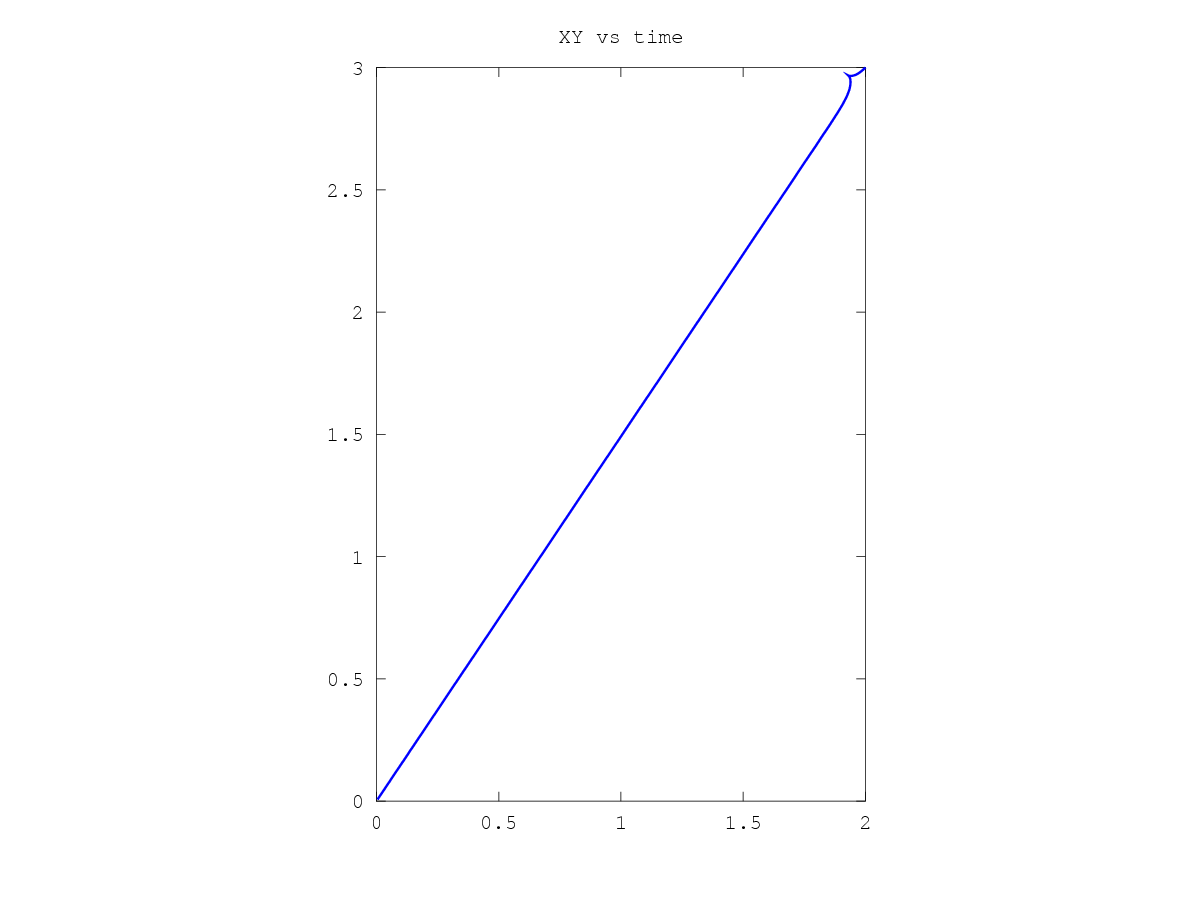
\includegraphics[scale=0.4]{figures/Question2b2Xyt.png} 
	          \label{fig:Q2b2Traj}
              }
              \subfigure[$x$ vs $t$ and $y$ vs $t$ ]{
	          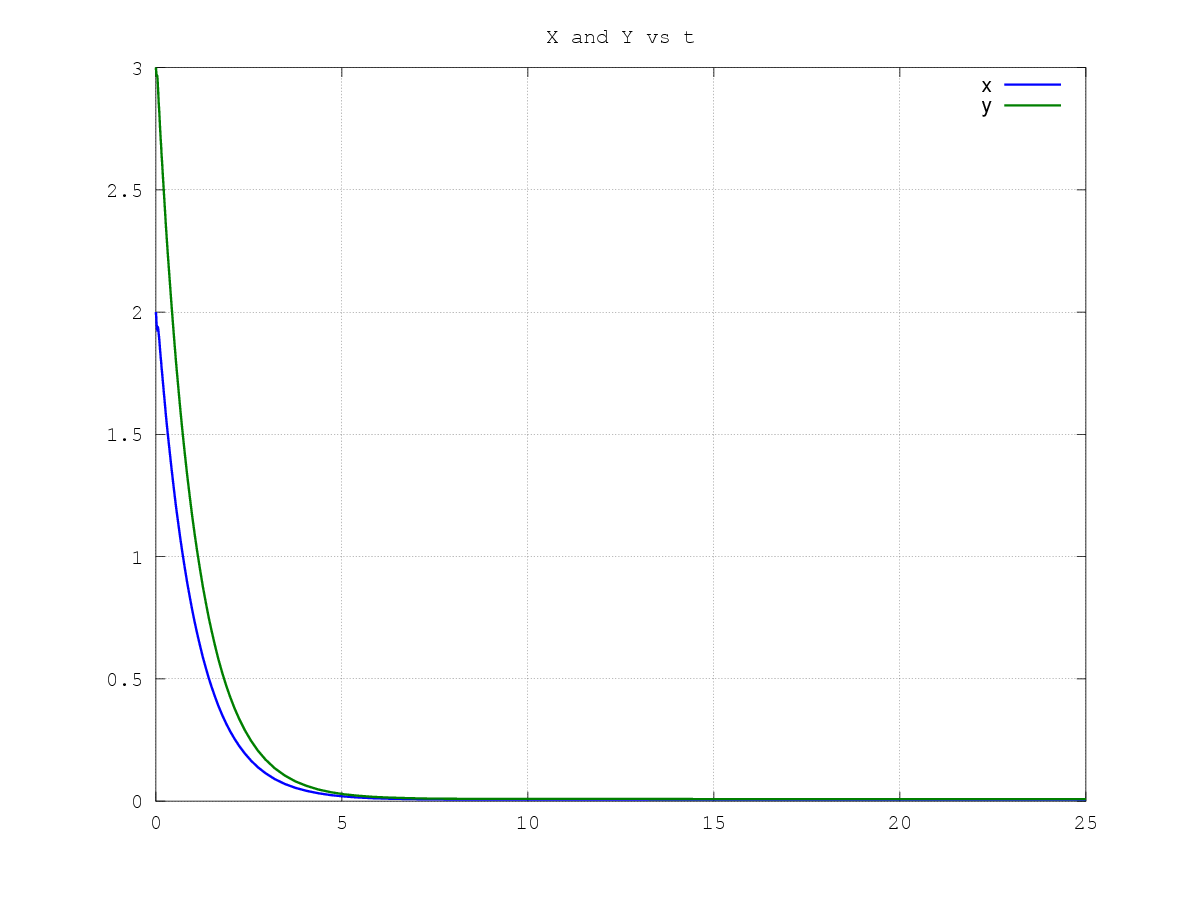
\includegraphics[scale=0.4]{figures/Question2b2Param.png} 	
	          \label{fig:Q2b2Xy}
              } 
            \caption{ Interesting Trajectory 2 }
            \label{fig:Q2b2}
	\end{figure}

% ---------------
\textbf{Initial Conditions 3:} $x_{0} = 2.0$, $y_{0} = 3.0$, $\theta = 7*\pi / 4 $, $\lambda_{0} = 0.5$
Here we try with a orientation pointing nearly opposite to the desired origin $\lambda$. The result is a path  with a circular section at the beginning, originated from the spinning of the robot to direct itself to the origin. Here the plots: 

	\begin{figure}[h]
			\centering
			  \subfigure[Parametric trajectory]{
			  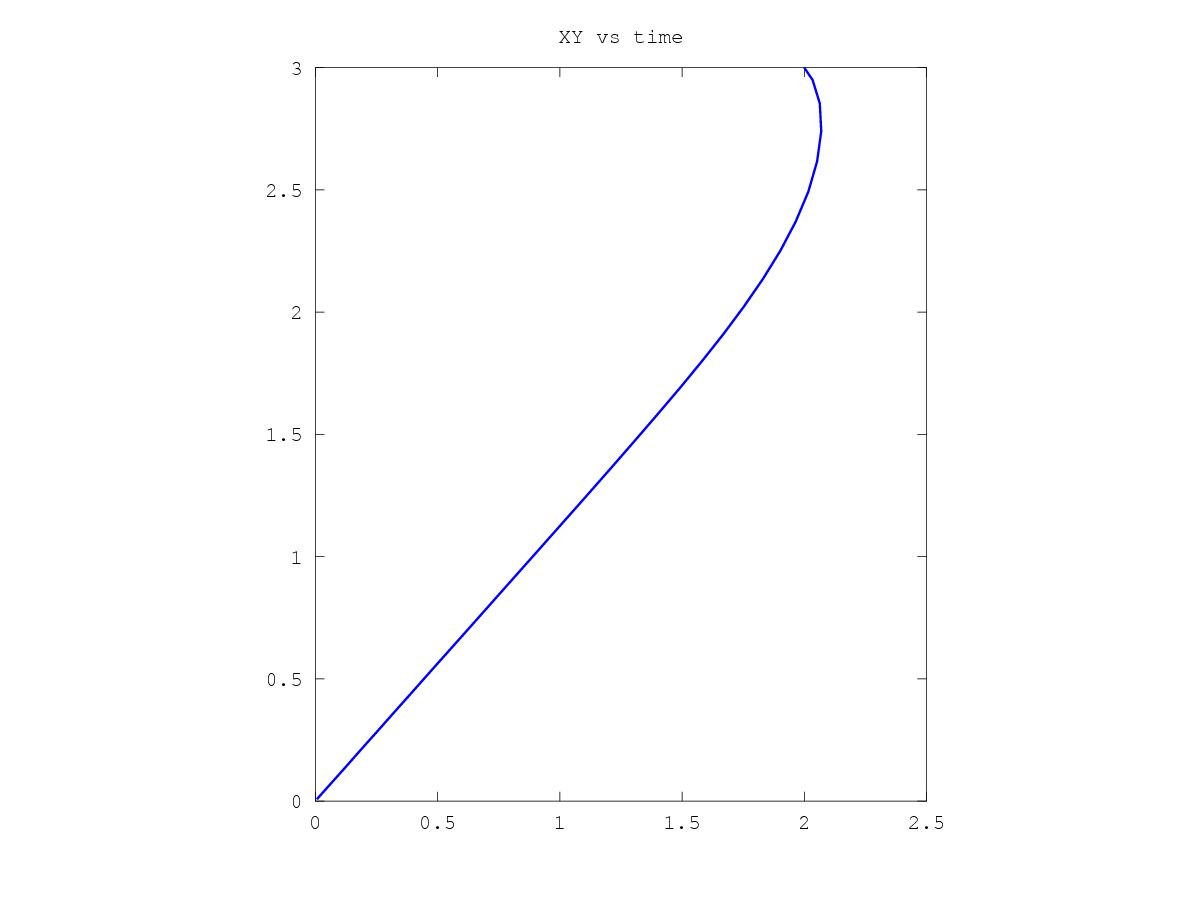
\includegraphics[scale=0.4]{figures/Question2b3Xyt.png} 
	          \label{fig:Q2b3Traj}
              }
              \subfigure[$x$ vs $t$ and $y$ vs $t$ ]{
	          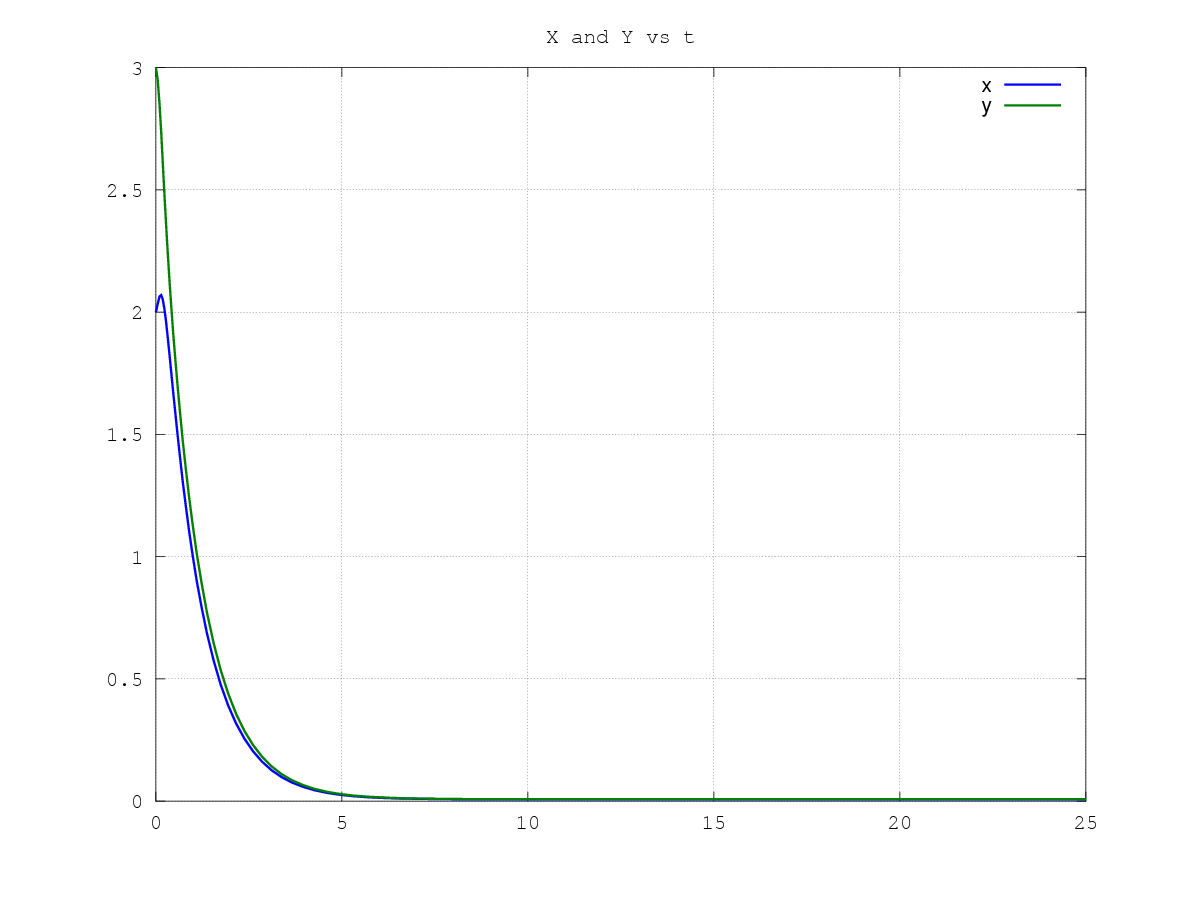
\includegraphics[scale=0.4]{figures/Question2b3Param.png} 	
	          \label{fig:Q2b3Xy}
              } 
            \caption{ Interesting Trajectory 3 }
            \label{fig:Q2b3}
	\end{figure}

% ---------------
\textbf{Initial Conditions 4:} $x_{0} = 2.0$, $y_{0} = 0.0$, $\theta = \pi / 2 $, $\lambda_{0} = 0.5$
Here we try with an initial position of $y = 0$. Due to the fact that $\lambda$ is neither too big, neither too small, the path is not a straight line but a curve. This  curve gets more pronounced if $\lambda$ is bigger and it gets more straight if $\lambda$ gets smaller. Here the plots:

	\begin{figure}[h]
			\centering
			  \subfigure[Parametric trajectory]{
			  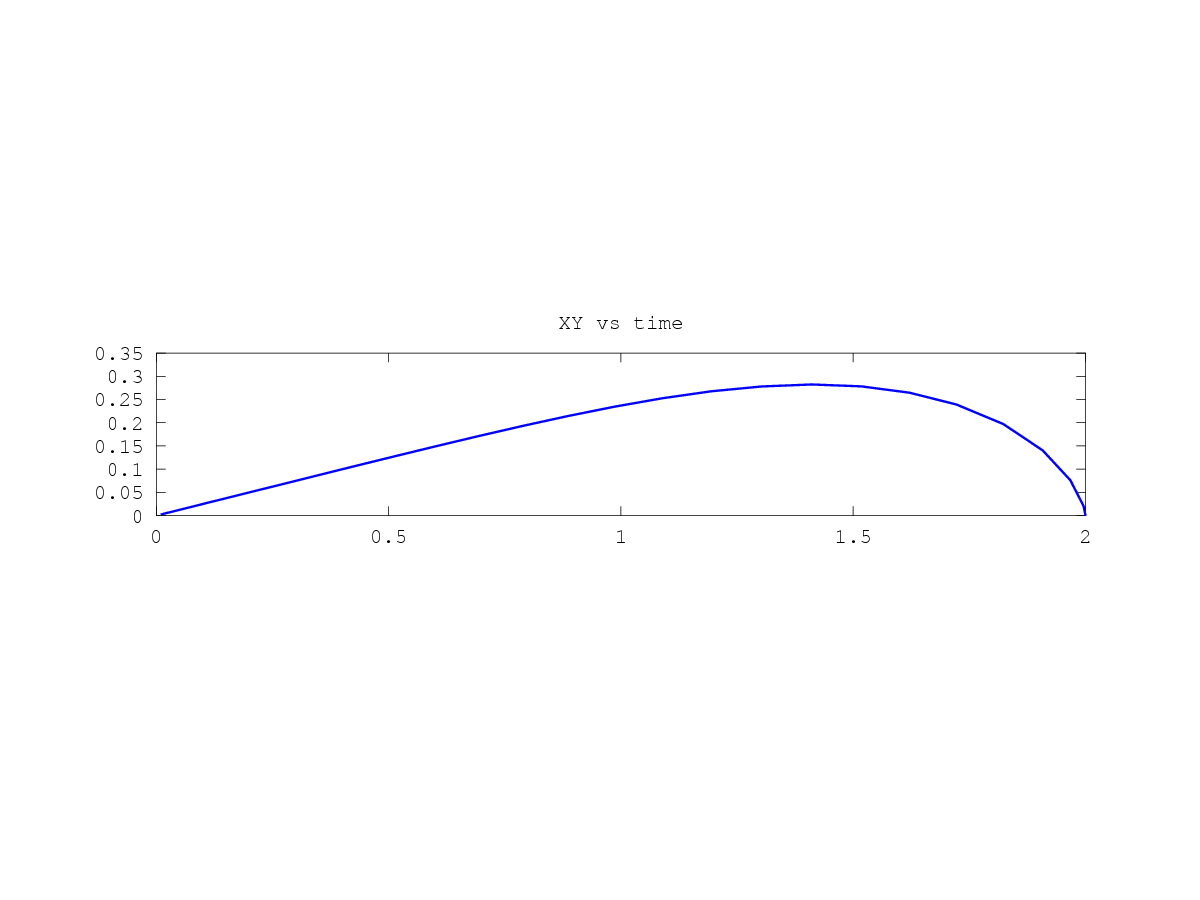
\includegraphics[scale=0.4]{figures/Question2b4Xyt.png} 
	          \label{fig:Q2b4Traj}
              }
              \subfigure[$x$ vs $t$ and $y$ vs $t$ ]{
	          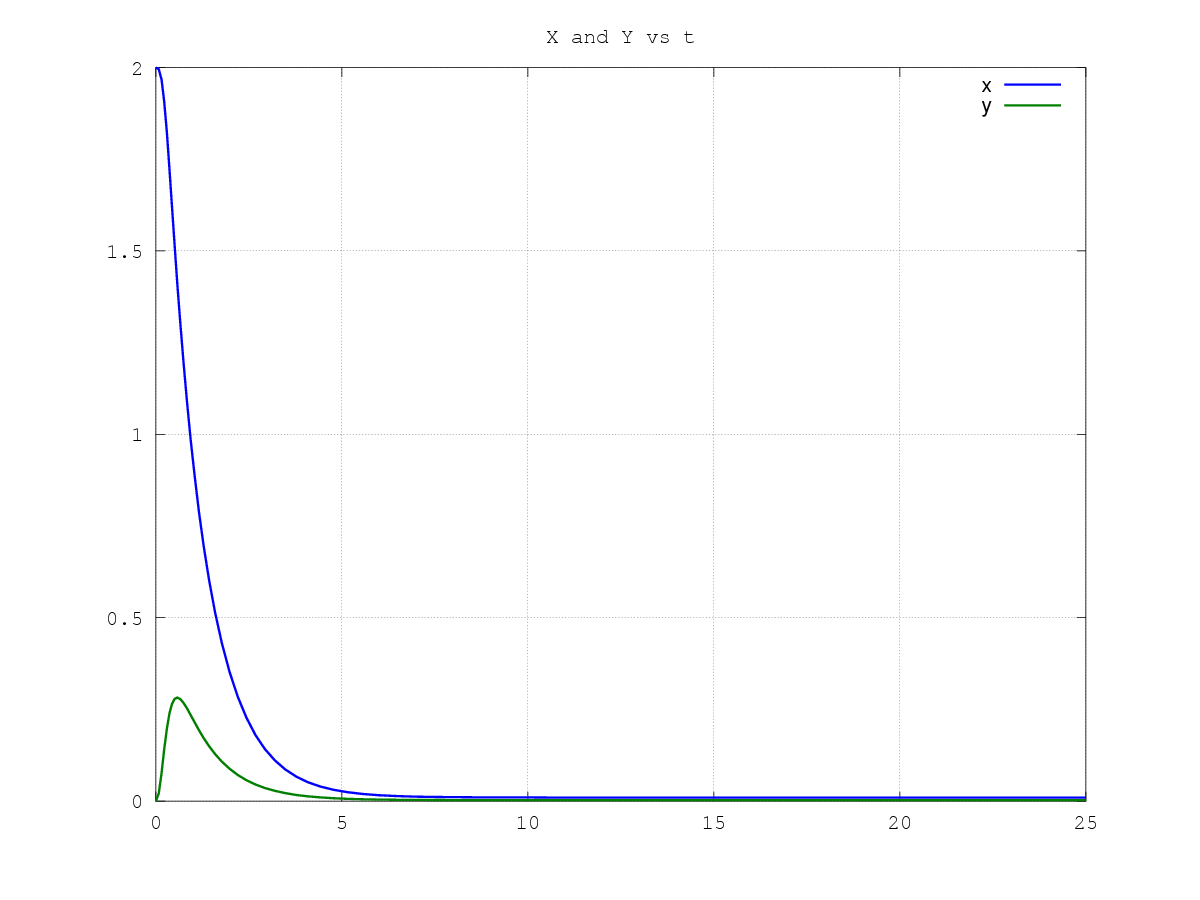
\includegraphics[scale=0.4]{figures/Question2b4Param.png} 	
	          \label{fig:Q2b4Xy}
              } 
            \caption{ Interesting Trajectory 4 }
            \label{fig:Q2b4}
	\end{figure}

\subsection*{(c)}
If you are ambitious, then you will try to track a trajectory. In that case, you need to do something like

\begin{center}
$\upsilon  = -Ke_{z}$ where $e_{z}(t) = z(t) - z_{des}(t)$
\end{center}

where $z_{des}(t)$ is directly obtained from the desired trajectory $g_{des}(t) = (x_{des}(t), y_{des}(t),\theta_{des}(t))$ (no transformation of coordinates, or think of it as $\lambda_{des} = 0$ with no feedback to drive $\lambda$ to $\lambda_{des}$). Notice that in spite of the lack of control on the $\theta$ variable, the system ends up doing the appropriate thing. This is what I said about how the system does what youy would do using common sense, but requires a fair amount of math to actually prove. The math could have been a little bit shorter, but not much more. You will not be graded for this part, it is just so you get comfortable with it, because this is probably the best controller you could do for trajectory tracking, plus changing the gains $K$ and $c$ have physical significance in terms of how the controller stabilizes.

\subsubsection*{Answer}
The easiest trajectory I could think of was one circle, so I ended up with the plots below (for the initial positions I put both $x$ and $y$ with some error with respect to the original. My plan was to track a circle of radius 2m. My final path indeed resembles a circle but of radius 1.5m, so seems I have to tune something there or I am doing something wrong :). My initial state was: $x= 2.3$, $y = 0.2$, $\theta = \pi/2$ and $\lambda = 0.02$ . Here the plots (luckily this is not graded :)

	\begin{figure}[h]
			\centering
			  \subfigure[Parametric trajectory]{
			  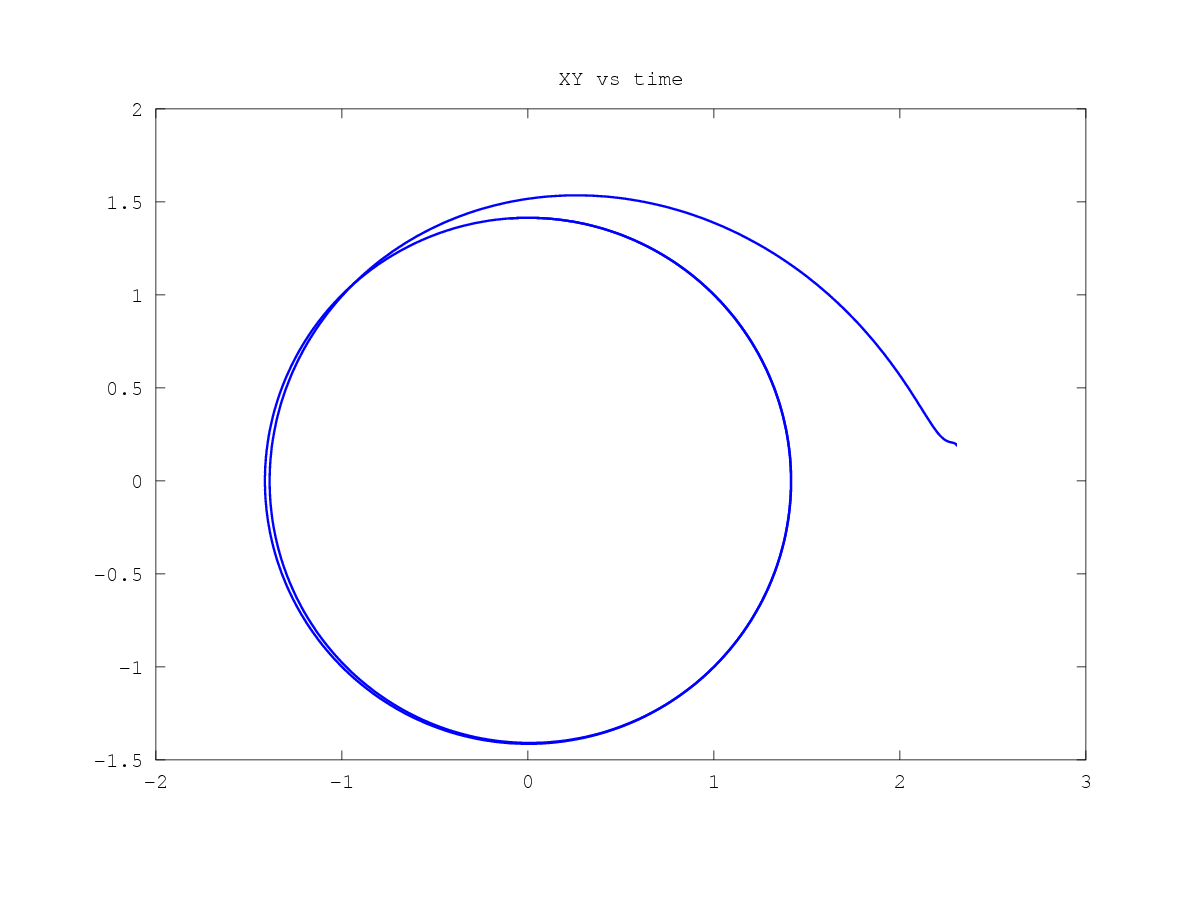
\includegraphics[scale=0.4]{figures/Question2cXyt.png} 
	          \label{fig:Q2cTraj}
              }
              \subfigure[$x$ vs $t$ and $y$ vs $t$ ]{
	          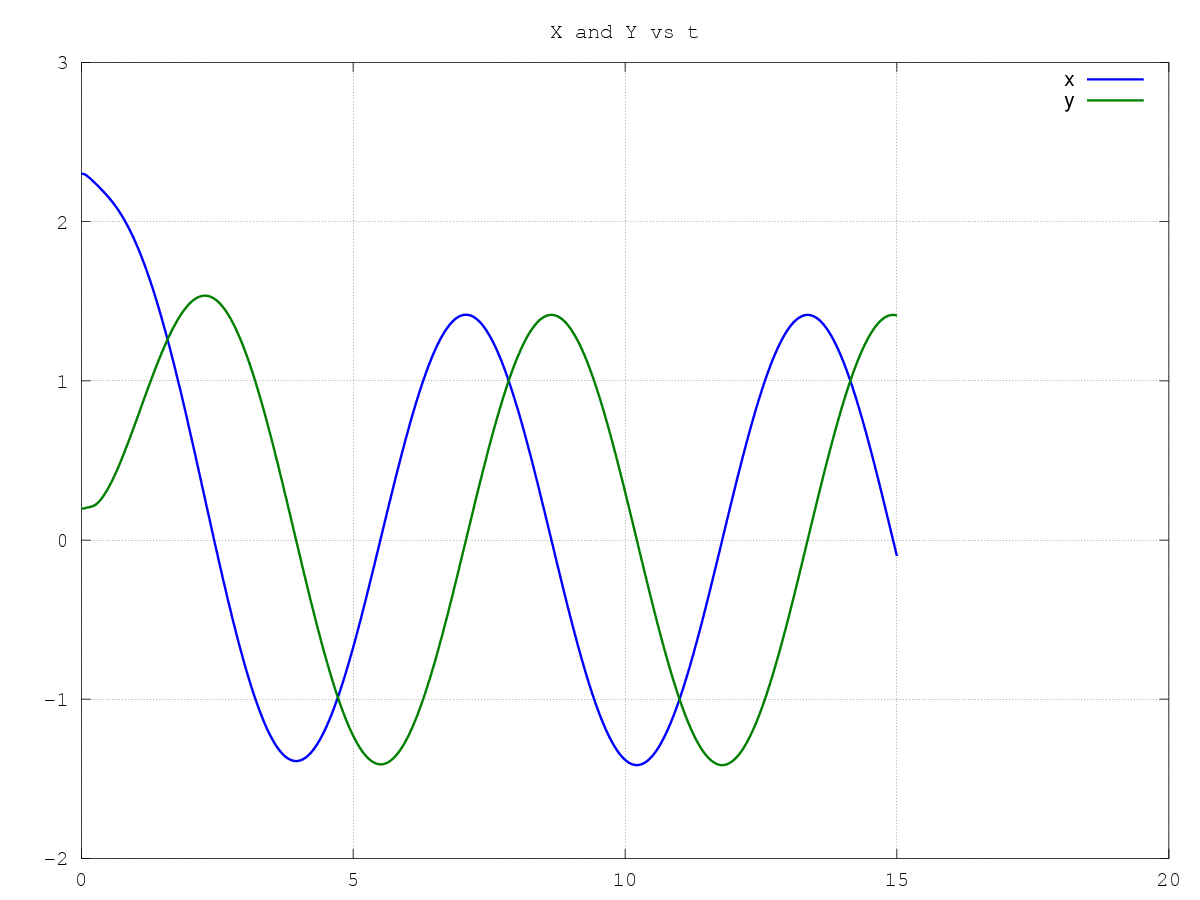
\includegraphics[scale=0.4]{figures/Question2cParam.png} 	
	          \label{fig:Q2cXy}
              } 
            \caption{ x vs t and y vs t }
            \label{fig:Q2c}
	\end{figure}
 
 
 
\end{document}